\documentclass[10pt]{beamer}

\usepackage{packages}
\title{Exercício Programa 2}
\subtitle{Corrida por eliminação}
\institute{IME-USP}
\author{Lucas Paiolla Forastiere, 11221911\\ Marcos Siolin Martins, 11221709}
\date{05 de novembro de 2020}

\begin{document}
    \maketitle

    \section{Detalhes de Implementação}

    \begin{frame}{Detalhes de Implementação - Os competidores}
        \begin{itemize}
            \justifying
            \item Cada ciclista possui uma \texttt{struct} própria com todas
                as informações necessárias para a corrida e as estatísticas;
            \item Essas \texttt{structs} ficam armazenadas em um vetor global
                chamado \texttt{ciclistas}.
            \item Enquanto isso, as threads de cada ciclista ficam em um vetor
                à parte chamado \texttt{threads}.

        \end{itemize}
    \end{frame}

    \begin{frame}{Detalhes de Implementação - A pista}
        \begin{itemize}
            \justifying
            \item A pista é uma matriz de inteiros com tamanho máximo de
                \texttt{D\_MAX (2000)} por \texttt{FAIXAS (10)}. Se
                \texttt{pista[i][j]} é $0$, então não há nenhum ciclista no
                metro $i$, faixa $j$, caso contrário, o número dessa posição é
                o ciclista que se encontra nela;
            \item Além disso, existe uma matriz \texttt{mutex\_pista} de mesmas
              dimensões com um \textit{mutex} para cada posição da pista.
        \end{itemize}
    \end{frame}

    \begin{frame}{Detalhes de Implementação - O movimento - 1}
      \begin{itemize}
        \justifying
        \item Cada ciclista é responsável por seu próprio movimento, liberando
          ou travando os \textit{mutexes} necessários. Sempre que precisamos
          checar uma posição da pista, travamos o \textit{mutex} correspondente,
          fazemos as verificações e depois o liberamos;
          \item Se a posição da frente está livre, então ele simplesmente anda
          para frente;
        \item Se ela está ocupada por um ciclista que ainda não fez sua ação,
          então esperamos por ele (liberando o seu \textit{mutex});
      \end{itemize}
    \end{frame}

    \begin{frame}{Detalhes de Implementação - O movimento - 2}
      \begin{itemize}
        \justifying
        \item Se ele está a mais que $30$ Km/h e não conseguiu andar para
          frente, então ele tenta ultrapassar (verificando as faixas mais
          externas). Na verificação, se ele não conseguir travar o
          \textit{mutex} por qualquer motivo, então tenta a próxima faixa mais
          externa;
      \end{itemize}
    \end{frame}

    \begin{frame}{Detalhes de Implementação - Turnos e Barreiras}
      \begin{itemize}
        \justifying
      \end{itemize}
    \end{frame}

    \begin{frame}{Arquitetura do Shell}
      Além disso algumas decisões de projetos foram tomadas, entre elas:
      \begin{itemize}
        \justifying
        \item A função \texttt{read\_command(command, parameters)} recebe a entrada digitada pelo usuário, usando a função \texttt{readline()}, e devolve o comando na variável \texttt{command} e cada parâmetro no vetor \texttt{parameters}. Por definição, \texttt{parameters[0] = command};
        \item A função \texttt{readline()} aloca a memória necessária. Guardamos seu retorno no histórico usando \texttt{add\_history()} e tratamos seu retorno substituindo espaços em branco pelo caractere `\textbackslash 0' e mudando os ponteiros de \texttt{parameters} para o começo de cada parâmetro na string.
      \end{itemize}
    \end{frame}
    \begin{frame}{Arquitetura do Shell}
      Antes do tratamento:
      \begin{figure}
        \begin{tikzpicture}
          \node at (-1,1) (command) {\texttt{command}};
          \node at (0,0) [square,draw,minimum size=0.75cm] (0) {l};
          \node at (0.75,0) [square,draw,minimum size=0.75cm] (1) {n};
          \node at (1.5,0) [square,draw,minimum size=0.75cm] (2) {};
          \node at (2.25,0) [square,draw,minimum size=0.75cm] (3) {-};
          \node at (3,0) [square,draw,minimum size=0.75cm] (4) {s};
          \node at (3.75,0) [square,draw,minimum size=0.75cm] (5) {};
          \node at (4.5,0) [square,draw,minimum size=0.75cm] (6) {a};
          \node at (5.25,0) [square,draw,minimum size=0.75cm] (7) {};
          \node at (6,0) [square,draw,minimum size=0.75cm] (8) {b};
          \node at (6.75,0) [square,draw,minimum size=0.75cm] (9) {\textbackslash 0};
          \draw[->] (command) edge[out=270,in=180] (0);
        \end{tikzpicture}
      \end{figure}
      Depois do tratamento:
      \begin{figure}
        \begin{tikzpicture}
          \node at (-1,1) (command) {\texttt{command}};
          \node at (-1,-1) (p0) {\texttt{parameters[0]}};
          \node at (2,1) (p1) {\texttt{parameters[1]}};
          \node at (3,-1) (p2) {\texttt{parameters[2]}};
          \node at (5,1) (p3) {\texttt{parameters[3]}};
          \node at (0,0) [square,draw,minimum size=0.75cm] (0) {l};
          \node at (0.75,0) [square,draw,minimum size=0.75cm] (1) {n};
          \node at (1.5,0) [square,draw,minimum size=0.75cm] (2) {\textbackslash 0};
          \node at (2.25,0) [square,draw,minimum size=0.75cm] (3) {-};
          \node at (3,0) [square,draw,minimum size=0.75cm] (4) {s};
          \node at (3.75,0) [square,draw,minimum size=0.75cm] (5) {\textbackslash 0};
          \node at (4.5,0) [square,draw,minimum size=0.75cm] (6) {a};
          \node at (5.25,0) [square,draw,minimum size=0.75cm] (7) {\textbackslash 0};
          \node at (6,0) [square,draw,minimum size=0.75cm] (8) {b};
          \node at (6.75,0) [square,draw,minimum size=0.75cm] (9) {\textbackslash 0};
          \draw[->] (command) edge[out=270,in=180] (0);
          \draw[->] (p0) edge[out=90,in=200] (0);
          \draw[->] (p1) edge[out=270,in=90] (3);
          \draw[->] (p2) edge[out=90,in=270] (6);
          \draw[->] (p3) edge[out=270,in=90] (8);
        \end{tikzpicture}
      \end{figure}
    \end{frame}
    \begin{frame}{Arquitetura do Shell}
      \begin{itemize}
        \justifying
        \item Todos os arrays que não são alocados por funções externas são alocados estaticamente com valor máximo definido por diretivas \texttt{\#define}:
        \begin{itemize}
          \vspace{-0.25in}
          \item \texttt{CUR\_DIR\_SIZE}: tamanho máximo do nome do diretório;
          \item \texttt{PROMPT\_SIZE}: tamanho máximo da string exibida no prompt;
          \item \texttt{MAX\_PARAMETERS}: quantidade máxima de parâmetros.
        \end{itemize}
        \item As syscalls utilizadas para os comandos internos foram \texttt{mkdir}, \texttt{symlink} e \texttt{kill}. Para a execução dos binários utilizamos a chamada \texttt{execve}.
        Na chamada de sistema \texttt{mkdir} passamos como parâmetro a
        constante \texttt{S\_IRWXU} que dá ao usuário todas as permissões
        sobre aquele diretório.
      \end{itemize}
    \end{frame}
    \section{Escalonadores}
    \subsection{Implementação}
    \begin{frame}{Implementação dos Escalonadores}
        \begin{itemize}
            \justifying
            \item Inicialmente, todas as threads que eventualmente chegarão no sistema são carregadas do arquivo de entrada, criadas e ficam bloqueadas até que o escalonador lhes dê a permissão de rodar.

            \item Para fazer esse gerenciamento das threads, existe um array de mutex (chamado \texttt{mutex}) em
        que cada mutex está associado a uma thread. Se o mutex está liberado, então a thread pode
        rodar. Caso contrário, a thread fica bloqueada.

            \item Usamos os mutex da biblioteca
        \texttt{pthread} para fazer esse gerenciamento, juntamente com as funções \texttt{pthread\_lock} e \texttt{pthread\_unlock}.
        \end{itemize}
    \end{frame}
    \begin{frame}{Implementação dos Escalonadores}
        \begin{itemize}
            \justifying
            \item A variável inteira chamada \texttt{semaforo} possui valor igual à thread que está em execução no momento (decidimos que apenas uma thread executaria por vez).

            \item Essa variável é gerenciada pela função \texttt{setSemaforo(value)},
        que recebe o valor da thread que executará e bloqueia a antiga
        thread para liberar a nova (caso o valor passado seja -1,
        então isso indica que nenhuma thread está em execução no momento).
        \end{itemize}
    \end{frame}

    \begin{frame}{Implementação dos Escalonadores}
        \begin{itemize}
            \justifying
            \item Decidimos também criar uma \texttt{struct} para os processos, para
        armazenar algumas informações de cada processo. Como o tempo em que ela terminou
        de executar e as propriedades informadas no arquivo de trace.

            \item Esses processos ficam em um array chamado \texttt{processos} que possui tamanho
        máximo igual a \texttt{nmax}. Assumimos que o número máximo de processos é
        $1000$, mas deixamos \texttt{nmax} como $1024$ para ter uma folga.

            \item Todas as variáveis e funções de uso amplo foram colocadas no arquivo
        \texttt{util.h} e cada escalonador foi implementado em um arquivo próprio.
        \end{itemize}
    \end{frame}

    \begin{frame}{Implementação dos Escalonadores}
        \begin{itemize}
                \justifying
                \item Por fim, o arquivo \texttt{ep1.c} possui a função \texttt{main} e a função
        \texttt{busy}, que é a função executada por cada uma das threads.

        \item O consumo de CPU realizado por ela advém da função \texttt{sched\_getcpu()},
        que retorna a CPU atual em que a thread está executando. Nos nossos testes,
        esse uso foi de $100\%$ do núcleo para os escalonadores \texttt{FCFS} e \texttt{SRTN}. Já no \texttt{round robin} a ocorrência massiva de preempções dificulta a visualização de qual CPU está sendo usada.
        \end{itemize}
    \end{frame}
    \begin{frame}{Implementação dos Escalonadores - Tempo}
        \begin{itemize}
            \justifying
            \item Sobre o tempo da simulação, o próprio escalonador controla o tempo passado
        através do uso da função \texttt{usleep(t)} que coloca o escalonador para ``dormir''
        por (pelo menos) $t$ microssegundos. Quando o escalonador ``acorda'' se passaram pelo
        menos $t$ microssegundos e assumimos que exatamente $t$ microssegundos se passaram (o erro cometido por \texttt{usleep} é pequeno de acordo com a documentação).

            \item A variável global \texttt{cur\_time} controla quantos segundos na simulação se passaram.
        Ela começa com valor igual ao $t_0$ do primeiro processo (avançamos a simulação para o ponto em que o primeiro processo chega).
        \end{itemize}
    \end{frame}
    \begin{frame}{Implementação dos Escalonadores - FCFS}
        \begin{itemize}
            \justifying
            \item No FCFS, aproveitamos a própria fila de processos carregada na entrada para
        simular a ordem dos processos.

        \item Usamos uma variável \texttt{atual} para controlar o índice da thread que
        está executando no momento e vamos atualizando o tempo que ela ficou
        executando conforma a simulação avança.

        \item Além disso, também mantemos uma variável \texttt{prox} para dizer qual é
        o próximo processo que vai chegar na simulação. Enquando o tempo atual da
        simulação é igual ao $t_0$ de \texttt{prox} indicamos a chegada dele e
        incrementamos a variável.
        \end{itemize}
    \end{frame}

    \begin{frame}{Implementação dos Escalonadores - SRTN}
        \begin{itemize}
            \justifying
            \item No SRTN, usamos um vetor \texttt{fila} que guarda os índices de cada thread.

            \item A variável \texttt{prox} tem o mesmo papel que no FCFS, assim como
        \texttt{atual}.

            \item A variável \texttt{ini} aponta para o começo da fila e, por definição,
        \texttt{fila[ini-1]} é o processo que está executando no momento.

            \item A variável \texttt{fim} aponta para a última posição não ocupada da fila e,
        por definição, \texttt{fila[fim]} é sempre igual a -1.

            \item Além disso, esse escalonador conta com a função \texttt{insere\_na\_fila}, que
        insere o processo que acabou de chegar no seu lugar apropriado na fila
        (ordenado pelo tempo restante de execução) e atualiza os valores de
        \texttt{ini} e \texttt{fim}.
        \end{itemize}
    \end{frame}

    \begin{frame}{Implementação dos Escalonadores - Round-Robin}
        \begin{itemize}
            \justifying
            \item No Round-Robin, a fila de processos carregada na entrada é reaproveitada para simular a ordem dos processos.

            \item As variáveis \texttt{atual} e \texttt{prox} cumprem o mesmo papel que dos outros dois escalonadores,
        enquanto a variável \texttt{tempo\_dormindo} controla quantos microssegundos além do segundo atual já se passaram.

            \item O \texttt{quantum} é definido em um \texttt{\#define} e é dado em microssegundos. Testamos para \texttt{quantum = 0.05s}.

            \item A variável \texttt{minimo} assegura que o escalonador não dormirá por \texttt{quantum} se o tempo para o processo terminar é menor que isso.

            \item A variável \texttt{todos\_terminaram} controla se todos os processos já encerraram sua execução.
        \end{itemize}
    \end{frame}
    \begin{frame}{Implementação dos escalonadores - Round Robin}
    Na nossa implementação de Round Robin a fila circula nos processos que já chegaram e caso um novo processo chegue é colocado após o processo que chegou anteriormente. Exemplo:
    \begin{figure}
      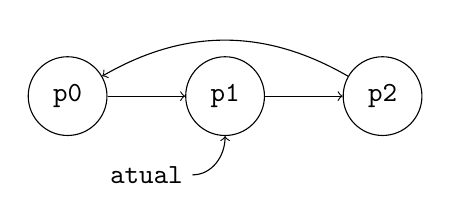
\begin{tikzpicture}
        \node at (0,0) [circle,draw, minimum size = 1cm] (0) {\texttt{p0}};
        \node at (2,0) [circle,draw, minimum size = 1cm] (1) {\texttt{p1}};
        \node at (4,0) [circle,draw, minimum size = 1cm] (2) {\texttt{p2}};
        \node at (1,-1) (at) {\texttt{atual}};
        \draw[->] (at) edge[out=0,in=270] (1);
        \draw[->] (0) -- (1);
        \draw[->] (1) -- (2);
        \draw[->] (2) edge[out = 150,in=30] (0);
      \end{tikzpicture}
    \end{figure}
    \begin{figure}
      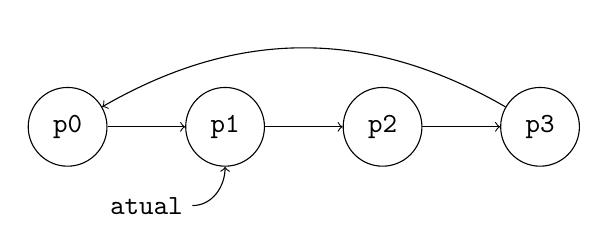
\begin{tikzpicture}
        \node at (0,0) [circle,draw, minimum size = 1cm] (0) {\texttt{p0}};
        \node at (2,0) [circle,draw, minimum size = 1cm] (1) {\texttt{p1}};
        \node at (4,0) [circle,draw, minimum size = 1cm] (2) {\texttt{p2}};
        \node at (6,0) [circle,draw, minimum size = 1cm] (3) {\texttt{p3}};
        \node at (1,-1) (at) {\texttt{atual}};
        \draw[->] (at) edge[out=0,in=270] (1);
        \draw[->] (0) -- (1);
        \draw[->] (1) -- (2);
        \draw[->] (2) -- (3);
        \draw[->] (3) edge[out = 150,in=30] (0);
      \end{tikzpicture}
    \end{figure}
    \end{frame}

    \subsection{Experimentos}
    \begin{frame}{Arquivo de Trace: 10 processos - Mudanças de contexto}
        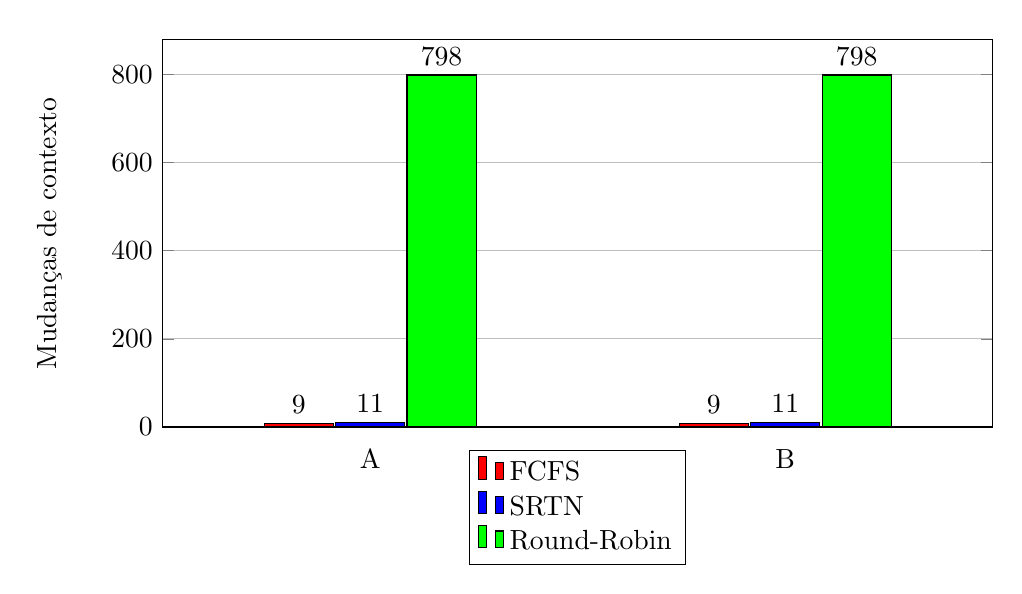
\begin{tikzpicture}
              \begin{axis}[
                  width  = 1.00*\textwidth,
                  height = 6.5cm,
                  major x tick style = transparent,
                  ylabel={Mudanças de contexto},
                  ylabel style={yshift=0.4cm},
                  ybar=2*\pgflinewidth,
                  bar width=25pt,
                  ymajorgrids = true,
                  symbolic x coords={A,B},
                  xtick = data,
                  scaled y ticks = false,
                  enlarge x limits=0.50,
                  ymin=0,
                  legend cell align=left,
                  legend style={at={(0.5,-0.06)},anchor=north},
                  nodes near coords,
                  nodes near coords align={anchor=south},%Move values in bar
                  totals/.style={nodes near coords align={anchor=north}},
                  x tick label style={anchor=south,yshift=-0.5cm},
              ]

              \addplot[style={fill=red},
                error bars/.cd,
                y dir=both,
                y explicit]
              coordinates {
                  (A, 9)
                  (B, 9)
              };

              \addplot[style={fill=blue},
                error bars/.cd,
                y dir=both,
                y explicit]
              coordinates {
                   (A, 11)
                   (B, 11)
              };

              \addplot[style={fill=green},
                error bars/.cd,
                y dir=both,
                y explicit]
              coordinates {
                   (A,798)
                   (B,798)
              };


              \legend{FCFS, SRTN, Round-Robin}
            \end{axis}
        \end{tikzpicture}
    \end{frame}

    \begin{frame}{Arquivo de Trace: 100 processos - Mudanças de contexto}
        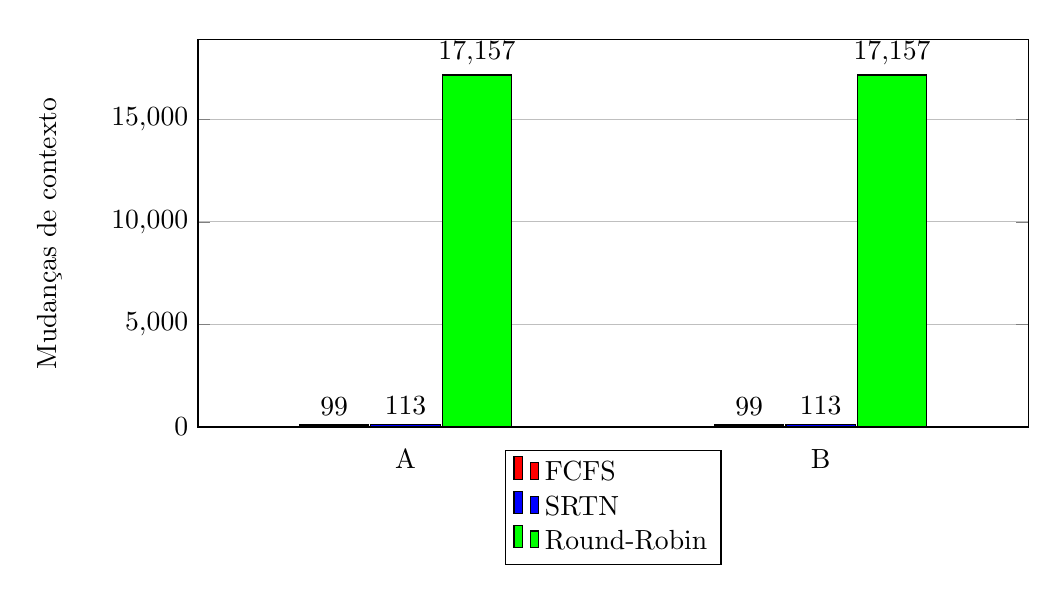
\begin{tikzpicture}
              \begin{axis}[
                  width  = 1.00*\textwidth,
                  height = 6.5cm,
                  major x tick style = transparent,
                  ylabel={Mudanças de contexto},
                  ylabel style={yshift=0.4cm},
                  ybar=2*\pgflinewidth,
                  bar width=25pt,
                  ymajorgrids = true,
                  symbolic x coords={A,B},
                  xtick = data,
                  scaled y ticks = false,
                  enlarge x limits=0.50,
                  ymin=0,
                  legend cell align=left,
                  legend style={at={(0.5,-0.06)},anchor=north},
                  nodes near coords,
                  nodes near coords align={anchor=south},%Move values in bar
                  totals/.style={nodes near coords align={anchor=north}},
                  x tick label style={anchor=south,yshift=-0.5cm},
              ]

              \addplot[style={fill=red},
                error bars/.cd,
                y dir=both,
                y explicit]
              coordinates {
                  (A, 99)
                  (B, 99)
              };

              \addplot[style={fill=blue},
                error bars/.cd,
                y dir=both,
                y explicit]
              coordinates {
                   (A,113)
                   (B,113)
              };

              \addplot[style={fill=green},
                error bars/.cd,
                y dir=both,
                y explicit]
              coordinates {
                   (A,17157)
                   (B,17157)
              };

              \legend{FCFS, SRTN, Round-Robin}
            \end{axis}
        \end{tikzpicture}
    \end{frame}

    \begin{frame}{Arquivo de Trace: 1000 processos - Mudanças de contexto}
        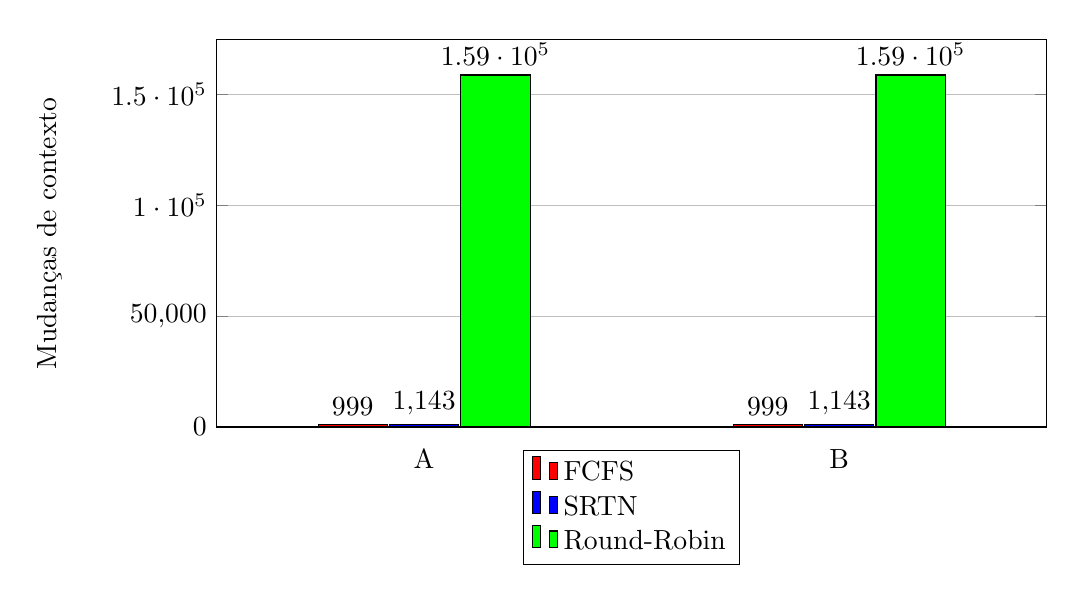
\begin{tikzpicture}
              \begin{axis}[
                  width  = 1.00*\textwidth,
                  height = 6.5cm,
                  major x tick style = transparent,
                  ylabel={Mudanças de contexto},
                  ylabel style={yshift=0.4cm},
                  ybar=2*\pgflinewidth,
                  bar width=25pt,
                  ymajorgrids = true,
                  symbolic x coords={A,B},
                  xtick = data,
                  scaled y ticks = false,
                  enlarge x limits=0.50,
                  ymin=0,
                  legend cell align=left,
                  legend style={at={(0.5,-0.06)},anchor=north},
                  nodes near coords,
                  nodes near coords align={anchor=south},%Move values in bar
                  totals/.style={nodes near coords align={anchor=north}},
                  x tick label style={anchor=south,yshift=-0.5cm},
              ]

              \addplot[style={fill=red},
                error bars/.cd,
                y dir=both,
                y explicit]
              coordinates {
                  (A, 999)
                  (B, 999)
              };

              \addplot[style={fill=blue},
                error bars/.cd,
                y dir=both,
                y explicit]
              coordinates {
                   (A,1143)
                   (B,1143)
              };

              \addplot[style={fill=green},
                error bars/.cd,
                y dir=both,
                y explicit]
              coordinates {
                   (A,158657)
                   (B,158657)
              };

              \legend{FCFS, SRTN, Round-Robin}
            \end{axis}
        \end{tikzpicture}
    \end{frame}
    \begin{frame}{Arquivo de Trace: 10 processos - Deadlines}
        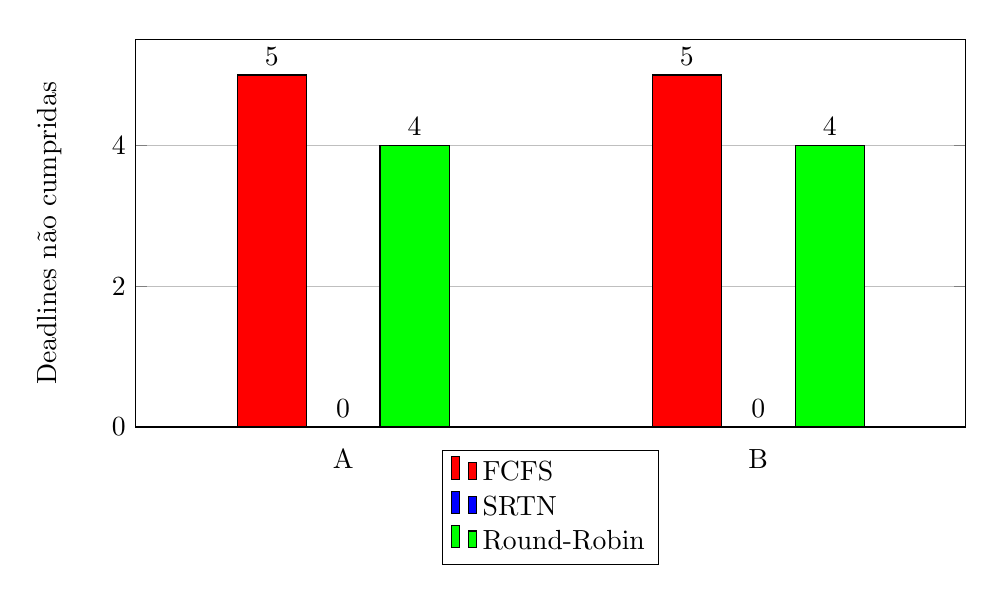
\begin{tikzpicture}
              \begin{axis}[
                  width  = 1.00*\textwidth,
                  height = 6.5cm,
                  major x tick style = transparent,
                  ylabel={Deadlines não cumpridas},
                  ylabel style={yshift=0.4cm},
                  ybar=2*\pgflinewidth,
                  bar width=25pt,
                  ymajorgrids = true,
                  symbolic x coords={A,B},
                  xtick = data,
                  scaled y ticks = false,
                  enlarge x limits=0.50,
                  ymin=0,
                  legend cell align=left,
                  legend style={at={(0.5,-0.06)},anchor=north},
                  nodes near coords,
                  nodes near coords align={anchor=south},%Move values in bar
                  totals/.style={nodes near coords align={anchor=north}},
                  x tick label style={anchor=south,yshift=-0.5cm},
              ]

              \addplot[style={fill=red},
                error bars/.cd,
                y dir=both,
                y explicit]
              coordinates {
                  (A, 5)
                  (B, 5)
              };

              \addplot[style={fill=blue},
                error bars/.cd,
                y dir=both,
                y explicit]
              coordinates {
                   (A, 0)
                   (B, 0)
              };

              \addplot[style={fill=green},
                error bars/.cd,
                y dir=both,
                y explicit]
              coordinates {
                   (A,4)
                   (B,4)
              };


              \legend{FCFS, SRTN, Round-Robin}
            \end{axis}
        \end{tikzpicture}
    \end{frame}

    \begin{frame}{Arquivo de Trace: 100 processos - Deadlines}
        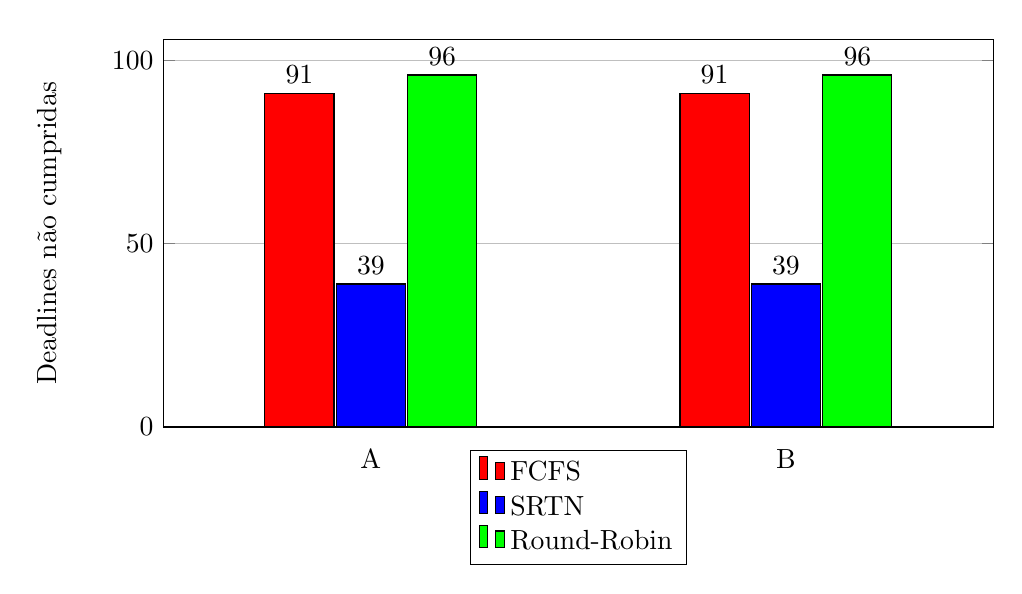
\begin{tikzpicture}
              \begin{axis}[
                  width  = 1.00*\textwidth,
                  height = 6.5cm,
                  major x tick style = transparent,
                  ylabel={Deadlines não cumpridas},
                  ylabel style={yshift=0.4cm},
                  ybar=2*\pgflinewidth,
                  bar width=25pt,
                  ymajorgrids = true,
                  symbolic x coords={A,B},
                  xtick = data,
                  scaled y ticks = false,
                  enlarge x limits=0.50,
                  ymin=0,
                  legend cell align=left,
                  legend style={at={(0.5,-0.06)},anchor=north},
                  nodes near coords,
                  nodes near coords align={anchor=south},%Move values in bar
                  totals/.style={nodes near coords align={anchor=north}},
                  x tick label style={anchor=south,yshift=-0.5cm},
              ]

              \addplot[style={fill=red},
                error bars/.cd,
                y dir=both,
                y explicit]
              coordinates {
                  (A, 91)
                  (B, 91)
              };

              \addplot[style={fill=blue},
                error bars/.cd,
                y dir=both,
                y explicit]
              coordinates {
                   (A,39)
                   (B,39)
              };

              \addplot[style={fill=green},
                error bars/.cd,
                y dir=both,
                y explicit]
              coordinates {
                   (A,96)
                   (B,96)
              };


              \legend{FCFS, SRTN, Round-Robin}
            \end{axis}
        \end{tikzpicture}
    \end{frame}

    \begin{frame}{Arquivo de Trace: 1000 processos - Deadlines}
        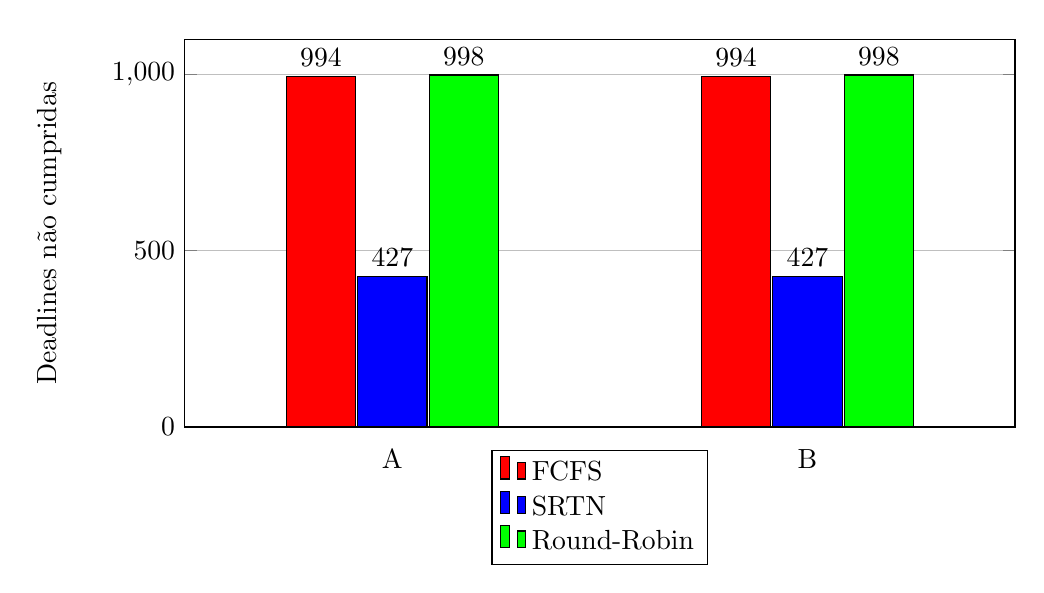
\begin{tikzpicture}
              \begin{axis}[
                  width  = 1.00*\textwidth,
                  height = 6.5cm,
                  major x tick style = transparent,
                  ylabel={Deadlines não cumpridas},
                  ylabel style={yshift=0.4cm},
                  ybar=2*\pgflinewidth,
                  bar width=25pt,
                  ymajorgrids = true,
                  symbolic x coords={A,B},
                  xtick = data,
                  scaled y ticks = false,
                  enlarge x limits=0.50,
                  ymin=0,
                  legend cell align=left,
                  legend style={at={(0.5,-0.06)},anchor=north},
                  nodes near coords,
                  nodes near coords align={anchor=south},%Move values in bar
                  totals/.style={nodes near coords align={anchor=north}},
                  x tick label style={anchor=south,yshift=-0.5cm},
              ]

              \addplot[style={fill=red},
                error bars/.cd,
                y dir=both,
                y explicit]
              coordinates {
                  (A, 994)
                  (B, 994)
              };

              \addplot[style={fill=blue},
                error bars/.cd,
                y dir=both,
                y explicit]
              coordinates {
                   (A,427)
                   (B,427)
              };

              \addplot[style={fill=green},
                error bars/.cd,
                y dir=both,
                y explicit]
              coordinates {
                   (A,998)
               (B,998)
              };


              \legend{FCFS, SRTN, Round-Robin}
            \end{axis}
        \end{tikzpicture}
    \end{frame}

    \begin{frame}{Observações antes das conclusões}
        \begin{itemize}
            \justifying
            \item O computador A possuia 8 núcleos e o computador B possuia 4;
            \item O arquivo de trace utilizado foi gerado sob as seguintes condições:
                \begin{enumerate}
                    \item O $t_0$ do primeiro processo é um número de 1 a 10;
                    \item O $t_0$ de qualquer outro processo é o $t_0$ do processo
                        anterior mais um número entre 0 e 15;
                    \item O \texttt{dt} é um valor entre 1 e 21, mas com probabilidade
                        maior de ser um valor mais baixo;
                    \item O \texttt{deadline} é a soma do $t_0$ do processo
                        mais seu \texttt{dt} vezes um número entre 2 e 7.
                \end{enumerate}
        \end{itemize}
    \end{frame}

    \begin{frame}{Observações antes das conclusões}
        \begin{itemize}
            \justifying
            \item As threads da biblioteca \texttt{pthread} automaticamente mudam
                de \textit{core} porque o escalonador do próprio SO produz essas
                mudanças.
            \item Nós imprimimos essas mudanças quando a opção \texttt{d} foi
                explicitada, mas não somamos as mudanças de contexto do SO às
                mudanças de contexto da nossa simulação.
        \end{itemize}
    \end{frame}

    \begin{frame}{Conclusões dos experimentos}
        \begin{itemize}
            \justifying
            \item Os gráficos para os dois computadores foram exatamente os mesmos,
                pois nossa implementação
                considerou uma simulação com um núcleo apenas, então a diferença em
                núcleos dos computadores não afetaria os resultados.
            \item Além disso, todos os 30 testes com mesmo trace e escalonador
                geraram os mesmos resultados. Esse comportamento é esperado,
                pois os algoritmos de escalonamento implementados são
                determinísticos. Isso é por conta tanto da maneira como controlamos
                o tempo, como pelo fato de só haver uma thread em execução por vez.
            \item Como o desvio padrão é nulo não existe
                intervalo de confiança.
        \end{itemize}
    \end{frame}

    \begin{frame}{Conclusões dos experimentos - Mudanças de Contexto}
        \begin{itemize}
            \justifying
            \item A quantidade de mudanças de contexto do Round-Robin
                foi muito maior que as do demais, como o esperado, pois
                o quantum é muito pequeno.
            \item A quantidade de mudanças de contexto do FCFS foi exatamente a
                esperada, pois elas ocorrem sempre que os processos terminam,
                exceto quando a fila de espera está vazia.
            \item A quantidade de mudanças de contexto do SRTN foi também dentro
                do esperado por conta das situações em que um processo
                chega na fila com tempo de execução menor que o tempo restante
                do executando.
        \end{itemize}
    \end{frame}
    \begin{frame}{Conclusões dos experimentos - Deadlines}
        \begin{itemize}
            \justifying
            \item O Round-Robin obteve muitas falhas de deadline. Achamos que isso
                se deve ao fato de que nosso gerador de trace faz com que os
                processos cheguem na fila com uma constância muito grande (sem
                intervalos de tempo grandes sem nenhum processo chegando na fila).
                Assim, o Round-Robin começa a acumular muitos processos na fila e
                os processos antigos precisam revezar o tempo de execução com
                processos que acabaram de chegar.
            \item Similarmente, o FCFS também cumpre poucos deadlines, pois os
                processos novos se acumulam e precisam esperar os antigos terminarem
                primeiro.
        \end{itemize}
    \end{frame}

    \begin{frame}
        \begin{itemize}
        \justifying
        \item Por fim, o SRTN parece ser bem melhor que os demais, pois ele é o
            único que prioriza de alguma forma os processos que terminam em
            menos tempo.

        \item Talvez se estivéssemos testando o Round-Robin ou o FCFS em um ambiente
            favorável, poderíamos ver eles cumprindo mais deadlines, mas, de fato, o
            esperado era que o SRTN fosse o melhor nesse quesito pelos motivos
            comentados.
        \end{itemize}
    \end{frame}

    \begin{frame}
        \centering
        {\huge Obrigado!}

        $\\$

        Lucas e Marcos

    \end{frame}
\end{document}
